\documentclass{article}


%package needed to make this output
\usepackage[utf8]{inputenc}
\usepackage[a4paper, total={5.5in, 10in}]{geometry}
\usepackage[absolute,overlay]{textpos}
\usepackage{hyperref}
\hypersetup{colorlinks = true, urlcolor= blue, linkcolor= blue}
\usepackage[table,xcdraw]{xcolor}
\usepackage{graphicx}
\usepackage{amsmath}
\usepackage{afterpage}
\usepackage{caption}



%new colors frequently used in the document
\definecolor{Bonanno}{RGB}{21, 181, 231}
\definecolor{Lucchese}{RGB}{255, 106, 73}
\definecolor{Colombo}{RGB}{27, 111, 83}
\definecolor{Gambino}{RGB}{140, 184, 0}
\definecolor{Genovese}{RGB}{145, 87, 145}
\definecolor{Pagine}{RGB}{237, 239, 255}
\definecolor{Titoli}{RGB}{255, 72, 0}
\definecolor{Paragrafi}{RGB}{110, 2, 168}



%title, authors and date
\title{\vspace{-50pt}\huge\textbf{The Five Families in a Net}}
\author{Tiziano Iannaccio \\ Gianluca Mecci \\ Mihaela Nedkova Naydenova}
\date{\today}



\begin{document}
\maketitle
\pagecolor{Pagine}
\thispagestyle{empty} %no page number



%top-page pic, used in everypage
\begin{figure}[t!]
\vspace{-250pt}
\centering
\includegraphics[width=600pt]{networkpic1.jpg}
\advance\leftskip-3.52cm
\end{figure}



%our graph, stylized and without background
\begin{figure}[h!]
\vspace{-25pt}
\centering
\includegraphics[width=500pt]{networkpic2.png}
\advance\leftskip-1.5cm
\end{figure}



\begin{textblock*}{5cm}(14cm,29cm) 
\textbf{Network Analytics, a.a. 2020/2021}
\end{textblock*}
\newpage



\hypersetup{linkcolor=black}



\begin{figure}[t!]
\vspace{-250pt}
\centering
\includegraphics[width=600pt]{networkpic1.jpg}
\advance\leftskip-3.52cm
\end{figure}



%interactive index
\tableofcontents
\addtocontents{toc}{\protect\rule{\textwidth}{2pt}\par}
\hypersetup{linkcolor=blue}
\newpage



\begin{figure}[t!]
\vspace{-250pt}
\centering
\includegraphics[width=600pt]{networkpic1.jpg}
\advance\leftskip-3.52cm
\end{figure}



\section*{\textcolor{Titoli}{Introduction}}
\addcontentsline{toc}{section}{\numberline{}Introduction}
The idea behind our project was to have the complete control over our net. For this reason, we decided to make our own dataframe node by node and edge by edge. We chose to represent the \href{https://en.wikipedia.org/wiki/Five_Families}{Five Families of New York}, one of the most (in)famous mob organization in history. We were mainly interested in the seven decades from the 20's to the 80's, in order to put our focus on the rise and the growth of each family, or more precisely the growth of the information about these organizations collected by the U.S. Government.
\vspace{30pt}



\subsection*{\textcolor{Titoli}{Making the data}}
\addcontentsline{toc}{subsection}{\numberline{}Making the data}
The only way to build a network that would have contained all the information we needed was to look for each member of the Five Families one-by-one, from the \href{https://en.wikipedia.org/wiki/Crime_boss}{bosses} all the way to the capos. For basic data, such as the hierarchy within each family or the most important figures (which we hoped would have become our hubs) we used \href{https://en.wikipedia.org/wiki/Main_Page}{Wikipedia}, while for most of the time we have counted on \href{https://mafia.wikia.org/wiki/Mafia_Wiki}{Mafia Wiki}, which is an online encyclopedia with information that (quote): \begin{quote}"ranges from the Mafia roots, to individual bosses and their operations, including noteworthy associated and/or related criminal figures/crime subjects".\end{quote}
The esiest way to build our network was to represent each mobster with a node. Each node is enriched by 17 attributes, which define every individual's family-status, period of activity and, of course, family of belonging. We decided to go for a mixed graph, in which every edge has his source in the lower-status-node and his target in the higher one. We also wanted to build a complete graph, and so we decided to connect each family boss who was member of the \href{https://en.wikipedia.org/wiki/The_Commission_(American_Mafia)}{Commission} (the \textit{governing body of the American Mafia}) at the same time. After deciding our graph's structure, we looked for ever mobster's period of activity and built an edge every time two nodes with the same family-attribute would have also had a different position in the family (for example, every capo of the 1945 is linked to his boss at that time). We used different weights to underline the hierarchical difference between two individuals. We thought about it as a logical choice while building the net, because if we consider any edge as a way for information to spread across the web, it seems clear that an underboss is more likely to share his ideas with a boss rather than a capo.
\vspace{30pt}



\subsection*{\textcolor{Titoli}{Fixing the bugs}}
\addcontentsline{toc}{subsection}{\numberline{}Fixing the bugs}
As we will see in the \hyperlink{Analysis}{last paragraph} of this introduction, we have decided to use \href{https://www.python.org/}{Python} for analyzing our data, but it was not as smooth as silk as we thought. On top of that, we had evident problems in making our spreadsheets fully compatible with \href{https://gephi.org/}{Gephi}. We had to add 130 edges to our previous edge table, because Gephi and Python do not share the same versatility. More precisely, there was no way to implement a mixed graph in Python, and so we built a direct graph that supported parallel edges. After that, we merged the parallel edges to create what works just like a mixed graph, but we will see this process in detail \hyperlink{Analysis}{later on}. On the other hand, Gephi gives us the opportunity to build a mixed graph, so we decided to go for the heavier edge table. If you want to recreate our graphs, you can easily access to the data we used by clicking on this \href{https://github.com/TizianoIannaccio/Network-Analytics}{link}.
\newpage



\subsection*{\textcolor{Titoli}{Visualization}}
\label{sec:Visualization}



\begin{figure}[t!]
\vspace{-250pt}
\centering
\includegraphics[width=600pt]{networkpic1.jpg}
\advance\leftskip-3.52cm
\end{figure}



\pagecolor{white}\afterpage{\pagecolor{Pagine}}
\addcontentsline{toc}{subsection}{\numberline{}Visualization}
Having completed the dataframes, we started using Gephi for both looking for bugs and trying different layouts for our graph. We had a lot of options because of the elevated number of attributes that we built-in. In the following sample we have distinguished each family with a different color while tagging each node with the Name-attribute. The chosen layout is \href{https://github.com/gephi/gephi/wiki/Fruchterman-Reingold}{"Fruchterman Reingold"} with a lable-adjust algorithm.



%our graph
\begin{figure}[hbt!]
\centering
\includegraphics[width=575pt]{graphscreen.JPG}
\advance\leftskip-3cm
\end{figure}



%graph's legend
\vspace{-50pt}
\begin{flushright}
\advance\rightskip-2cm
\color{Lucchese}
\textbf{Lucchese Family}\\
\color{Genovese}
\textbf{Genovese Family}\\
\color{Gambino}
\textbf{Gambino Family}\\
\color{Colombo}
\textbf{Colombo Family}\\
\color{Bonanno}
\textbf{Bonanno Family}
\end{flushright}
\newpage



\subsection*{\hypertarget{Hierarchy}{\textcolor{Titoli}{Hierarchy}}}
\addcontentsline{toc}{subsection}{\numberline{}Hierarchy}



\begin{figure}[t!]
\vspace{-250pt}
\centering
\includegraphics[width=600pt]{networkpic1.jpg}
\advance\leftskip-3.52cm
\end{figure}



The following scheme explains how each family is structured and can be really helpful in understanding some choices in our network, such as the assignment of weights to the edges.



%the hierarchy three
\begin{figure}[!ht]
\centering
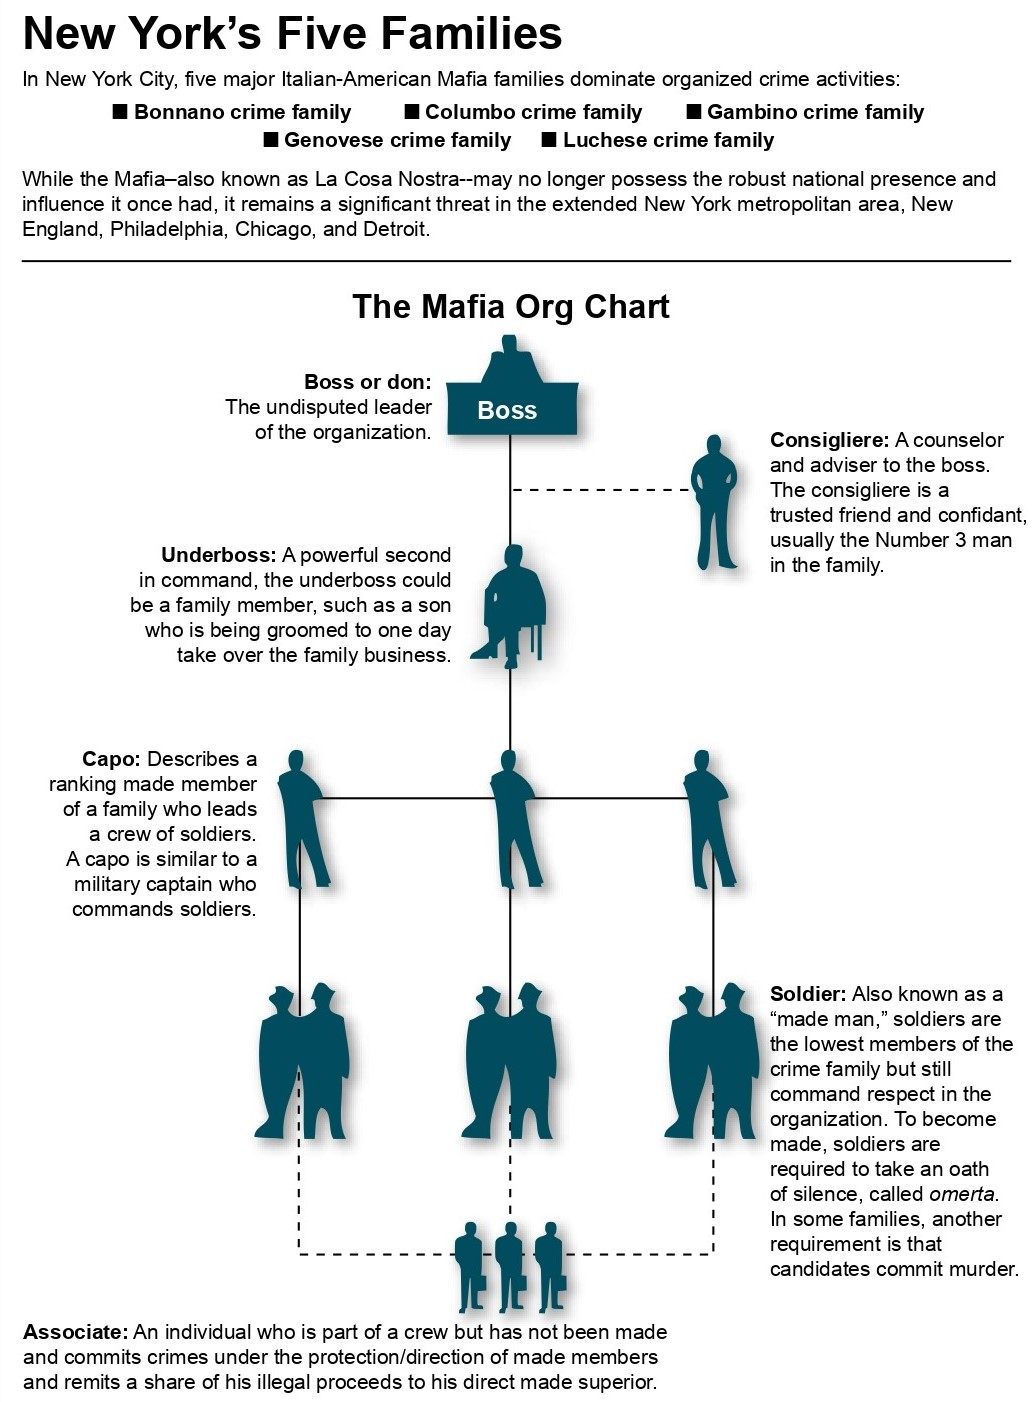
\includegraphics[width=400pt]{mafia-hierarchy.jpg}
\end{figure}
\newpage
\pagecolor{white}



\begin{figure}[t!]
\vspace{-250pt}
\centering
\includegraphics[width=600pt]{networkpic1.jpg}
\advance\leftskip-3.52cm
\end{figure}



\subsection*{\hypertarget{Analysis}{\textcolor{Titoli}{Analysis}}}
\addcontentsline{toc}{subsection}{\numberline{}Analysis}
As anticipated, our analysis was made mainly on Python, by using the following packages:
\begin{itemize}
    \item \href{https://matplotlib.org/stable/api/_as_gen/matplotlib.pyplot.html}{Matplotlib.pyplot} to show the graphs
    \item \href{https://numpy.org/}{NumPy} to have more powerful mathematical tools
    \item \href{https://networkx.org/}{NetworkX} to create our network
    \item \href{https://openpyxl.readthedocs.io/en/stable/}{OpenPyXL} to manipulate the node and edge tables
\end{itemize}
First of all, here's an overview of all the families in terms of nodes and edges:



%table with basic information
\begin{table}[h]
\advance\leftskip-0.6cm
\begin{tabular}{|l|l|l|l|l|l|l|}
\hline
\rowcolor[HTML]{DAE8FC} 
\multicolumn{1}{|c|}{\cellcolor[HTML]{DAE8FC}} & \multicolumn{1}{c|}{\cellcolor[HTML]{DAE8FC}\textbf{Bonanno}} & \textbf{Gambino} & \multicolumn{1}{c|}{\cellcolor[HTML]{DAE8FC}\textbf{Colombo}} & \textbf{Lucchese} & \textbf{Genovese} & \textbf{All the families} \\ \hline
\rowcolor[HTML]{ECF4FF} 
\cellcolor[HTML]{DAE8FC}\textbf{Edges} & 184 & 285 & 170 & 178 & 239 & 1317 \\ \hline
\rowcolor[HTML]{ECF4FF} 
\cellcolor[HTML]{DAE8FC}\textbf{Nodes} & 47 & 47 & 33 & 36 & 51 & 214 \\ \hline
\end{tabular}
\end{table}



\noindent
The sum of every family's edges does not add up to 1317 because it does not include any edge between members of different families.\\
We can already extrapolate a few information from this table:
\begin{itemize}
    \item There is a balance between each family in terms of high-profile figures
    \item The U.S. Government managed to get more information about the Gambino and the Genovese families
\end{itemize}
As anticipated, the analysis was not easy because NetworkX does not include the same functions of \textit{Graph} in \textit{MultiDiGraph}. We had to buid our own functions when possible and use Gephi for simple operations, like finding the network diameter, which is not possible with NetworkX while working on a "multi directed graph".\\
We highly recommend to try our interactive analysis program, which can be easily applied to most networks by simply changing the position of the spreadsheets and the name of each dictionary (attribute). The code for the analysis can be downloaded from this \href{https://github.com/TizianoIannaccio/Network-Analytics}{link}.\\
\vspace{-10pt}



\section{\textcolor{Paragrafi}{Degree distribution}}



%divides the page in 2 columns
\noindent\begin{minipage}{0.5\textwidth}
\advance\leftskip-3.3cm
\includegraphics[width=300pt]{degreehist.jpeg}
\end{minipage}%
\hfill%
\begin{minipage}{0.6\textwidth}\raggedleft
This histogram shows the degree distribution of our network. The first thing that jumps out is that a lot of nodes have a value of k (degree) between 1 and 20, while fewer nodes have a higher value of k. This behaviour is peculiar to the \href{https://en.wikipedia.org/wiki/Scale-free_network}{Scale-free networks}, while \href{https://en.wikipedia.org/wiki/Random_graph}{Random networks} tends to have a degree distribution centralized on the average degree . In our case, the nodes with a small value of k are the ones that represent the lowest point of the \hyperlink{Hierarchy}{hierarchy three}. For the same reason, the nodes with the highest degree are related to the bosses, which have a lot of connections. 
\end{minipage}
\newpage



\begin{figure}[t!]
\vspace{-250pt}
\centering
\includegraphics[width=600pt]{networkpic1.jpg}
\advance\leftskip-3.52cm
\end{figure}



\noindent\begin{minipage}{0.5\textwidth}
\advance\leftskip-3.3cm
\includegraphics[width=300pt]{scatterplot.jpeg}
\end{minipage}%
\hfill%
\begin{minipage}{0.6\textwidth}\raggedleft
This scatterplot (loglogplot) is a further confirm that our graph behaves as a Scale-free network. In contrast to a Random network, which would have presented a Poisson distribution, this plot resemble a power-law, even if the maximum degree is not that high. If we would analyze the values of $\gamma$, representing the exponent of the power-law, we would probably not see a value between 2 and 3, which is typical of the Scale-free networks. The easiest explanation to this apparent contradiction can be found in the small value of N in our network, meaning that 214 nodes are not enough to show the properties we talked about.
\end{minipage}



\vspace{30pt}
\noindent
The following picture shows our network's hubs. We decided to cut out every node with $k<30$. It is interesting to see that this subgraph is still connected, which helps reducing the average path length to 3.195. A logical observation is that the vast majority of the hubs represents a boss, connected to each member of his family at the time he is in charge of it. 



%our graphs hubs
\begin{figure}[!ht]
\centering
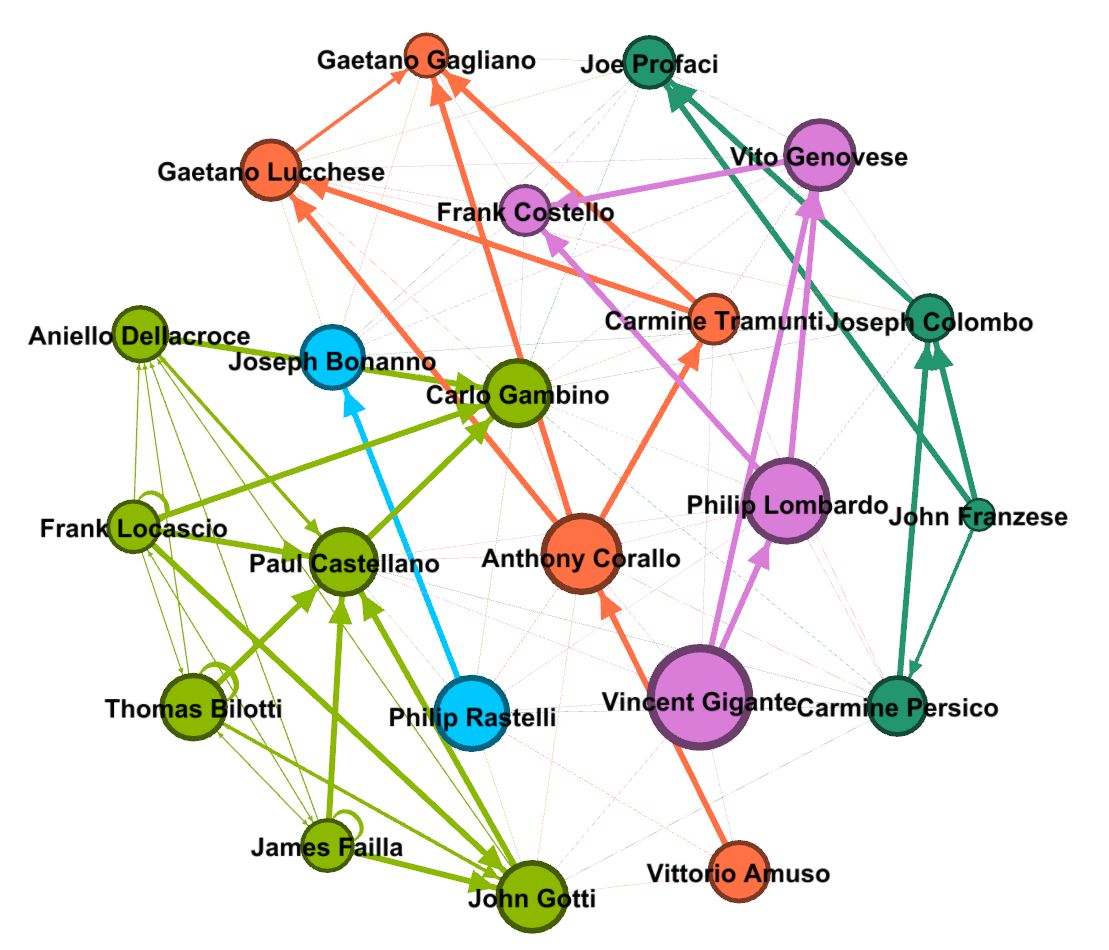
\includegraphics[width=350pt]{fullhubs.jpg}
\advance\leftskip-0.6cm
\end{figure}



\newpage
\begin{figure}[t!]
\vspace{-250pt}
\centering
\includegraphics[width=600pt]{networkpic1.jpg}
\advance\leftskip-3.52cm
\end{figure}



\section{\textcolor{Paragrafi}{Main descriptive measures}}
\pagecolor{Pagine}
It is now time to show some structural indices.
\textcolor{Titoli}{\subsection{Density, Diameter, Avg. Degree and Clustering Coefficient}}



%table with main indexes
\begin{table}[!h]
\advance\leftskip-1.8cm
\begin{tabular}{|l|c|c|c|c|c|c|}
\hline
\rowcolor[HTML]{DAE8FC} 
{\color[HTML]{FFFFFF} } & \multicolumn{1}{l|}{\cellcolor[HTML]{DAE8FC}{\color[HTML]{000000} \textbf{Bonanno}}} & \multicolumn{1}{l|}{\cellcolor[HTML]{DAE8FC}{\color[HTML]{000000} \textbf{Gambino}}} & \multicolumn{1}{l|}{\cellcolor[HTML]{DAE8FC}{\color[HTML]{000000} \textbf{Colombo}}} & \multicolumn{1}{l|}{\cellcolor[HTML]{DAE8FC}{\color[HTML]{000000} \textbf{Lucchese}}} & \multicolumn{1}{l|}{\cellcolor[HTML]{DAE8FC}{\color[HTML]{000000} \textbf{Genovese}}} & \multicolumn{1}{l|}{\cellcolor[HTML]{DAE8FC}{\color[HTML]{000000} \textbf{All the families}}} \\ \hline
\rowcolor[HTML]{ECF4FF} 
\cellcolor[HTML]{DAE8FC}{\color[HTML]{000000} \textbf{Graph Density}} & {\color[HTML]{000000} 0.085} & {\color[HTML]{000000} 0.132} & {\color[HTML]{000000} 0.162} & {\color[HTML]{000000} 0.141} & {\color[HTML]{000000} 0.094} & {\color[HTML]{000000} 0.029} \\ \hline
\rowcolor[HTML]{ECF4FF} 
\cellcolor[HTML]{DAE8FC}{\color[HTML]{000000} \textbf{Network Diameter}} & {\color[HTML]{000000} 6} & {\color[HTML]{000000} 4} & {\color[HTML]{000000} 5} & {\color[HTML]{000000} 4} & {\color[HTML]{000000} 4} & {\color[HTML]{000000} 8} \\ \hline
\rowcolor[HTML]{ECF4FF} 
\cellcolor[HTML]{DAE8FC}{\color[HTML]{000000} \textbf{Average Degree}} & {\color[HTML]{000000} 3.915} & {\color[HTML]{000000} 6.064} & {\color[HTML]{000000} 5.182} & {\color[HTML]{000000} 4.944} & {\color[HTML]{000000} 4.686} & {\color[HTML]{000000} 6.154} \\ \hline
\rowcolor[HTML]{ECF4FF} 
\cellcolor[HTML]{DAE8FC}{\color[HTML]{000000} \textbf{Clustering Coefficient}} & {\color[HTML]{000000} 0.296} & {\color[HTML]{000000} 0.373} & {\color[HTML]{000000} 0.344} & {\color[HTML]{000000} 0.429} & {\color[HTML]{000000} 0.388} & {\color[HTML]{000000} 0.38} \\ \hline
\end{tabular}
\end{table}



\begin{itemize}
    \item The \textbf{Graph Density} - the ratio between $L$ (number of links) and $L_{MAX}$ (number of links if the graph was complete). It is useful to understand if a graph is close to a complete network or not.
    \item The \textbf{Network Diameter} - the maximum distance between two nodes in the graph. In our case, the graph is directed and there is no way to go from certain nodes to others, and the diameter is for sure the distance between a capo of a random family and a boss of another family, passing through the bosses of every other family first.
    \item The \textbf{Average Degree} - The number of nodes to which each node is connected, in average.
    \item The \textbf{Average Clustering Coefficient} - The average of each node's clustering coefficient, obtainable from the following formula: 
\begin{equation*}
    \centering \scalebox{2}{$\frac{2L_i}{k_i(k_i-1)}$}
\end{equation*}
    \item[] where $L_i$ is the number of neighbors that $i$ shares with his own neighbors.
\end{itemize}



\noindent
Based on this data, the networks are strongly sparse, which is logical because, for example, not a single capo is linked to any other capo.\\
The Network Diameter is a clear reflection of the hierarchical structure of the families.\\
The Average Degree of each family range from 3.9 to 6, while for the full network surpasses 6.1, thanks to the newly gained connections between bosses of different families from the same period of time. The difference between, for example, the Gambino's and the Bonanno's value can be the result of 2 different causes:
\begin{itemize}
    \item The Gambino family was composed by more members of different status.
    \item The Bonanno family leaked less information.\\
\end{itemize}



\noindent
As we can see, the average Clustering Coefficient ranges from 0.3 to 0.4, a small value which tells us that for each node, the probability of his neighbors to be linked each other is fairly low. This value would have changed dramatically if we decided to link individuals with the same status within the family, because we would have formed a lot of triangles and the Average Clustering Coefficient would have been close to 1. 
\newpage
\pagecolor{white}



\begin{figure}[t!]
\vspace{-250pt}
\centering
\includegraphics[width=600pt]{networkpic1.jpg}
\advance\leftskip-3.52cm
\end{figure}



\section{\textcolor{Paragrafi}{Centrality measures}}
The centrality measures are used to understand which nodes are in a more strategic position of the network. In order to get these information, we used the NetworkX's functions \textit{degree\_centrality} and \textit{closeness\_centrality}. First of all, we initialized a variable by sorting the result of these functions applied to our graph. After that, we separated the identities from their values in order to implement in our charts each node's name as a label. We decided to include only the ten characters with the highest value (about 5\% of the total number of nodes) in a barplot, giving to each bar the color of this family, as shown in the \hyperref[sec:Visualization]{Visualization}.
\vspace{10pt}



\textcolor{Titoli}{\subsection{Degree centrality}}
First of all, we decided to analize the degree-centrality, because we wanted to find which mobster was more relevant to his own family. The degree-centrality is the most suitable index for this kind of analysis, because it is a purely local measure. \\



%output of ouor program
\begin{figure}[hbt!]
\centering
\advance\leftskip-5cm
\includegraphics[width=675pt]{centralchar.jpeg}
\end{figure}



\vspace{20pt}
\noindent
It is crucial to underline that the information about each family was not there for all to see, meaning that the more a boss was in charge of his family, the more occasions the FBI had to understand the dynamics of his figure. This consideration can be proved by the graph above, which at the highest positions does not show each family's founder, but the individuals with more decades of towing the family on their shoulders. In facts, the highest position obtained by a family founder is Carlo Gambino's 5th position. For instance, Vincent Gigante stayed on the bottom of the three from the 50's all the way to the 80's, the last decade of our research, but after that he became boss of his family from the 80's to the year of his death, in 2005. With more than 60 years of illegitimate activities, it is clear that he is the perfect "output" for our program. 
\newpage



\begin{figure}[t!]
\vspace{-250pt}
\centering
\includegraphics[width=600pt]{networkpic1.jpg}
\advance\leftskip-3.52cm
\end{figure}



\textcolor{Titoli}{\subsection{Closeness centrality}}
Due to the fact that it is not possible to calculate the \href{https://en.wikipedia.org/wiki/Betweenness_centrality}{betweenness centrality} for a Multi Directed Graph, we continued our analysis by calculating the closeness centrality. It is the reciprocal of the sum of the length of the shortest paths between the node and all other nodes in the graph, as shown in the following formula:
\begin{equation*}
    \scalebox{1.5}{$C(i) = \frac{n-1}{\sum_{j=1}^{n-1}d(j,i)}$}
\end{equation*}



\begin{figure}[h!]
\vspace{-20pt}
\centering
\advance\leftskip-5cm
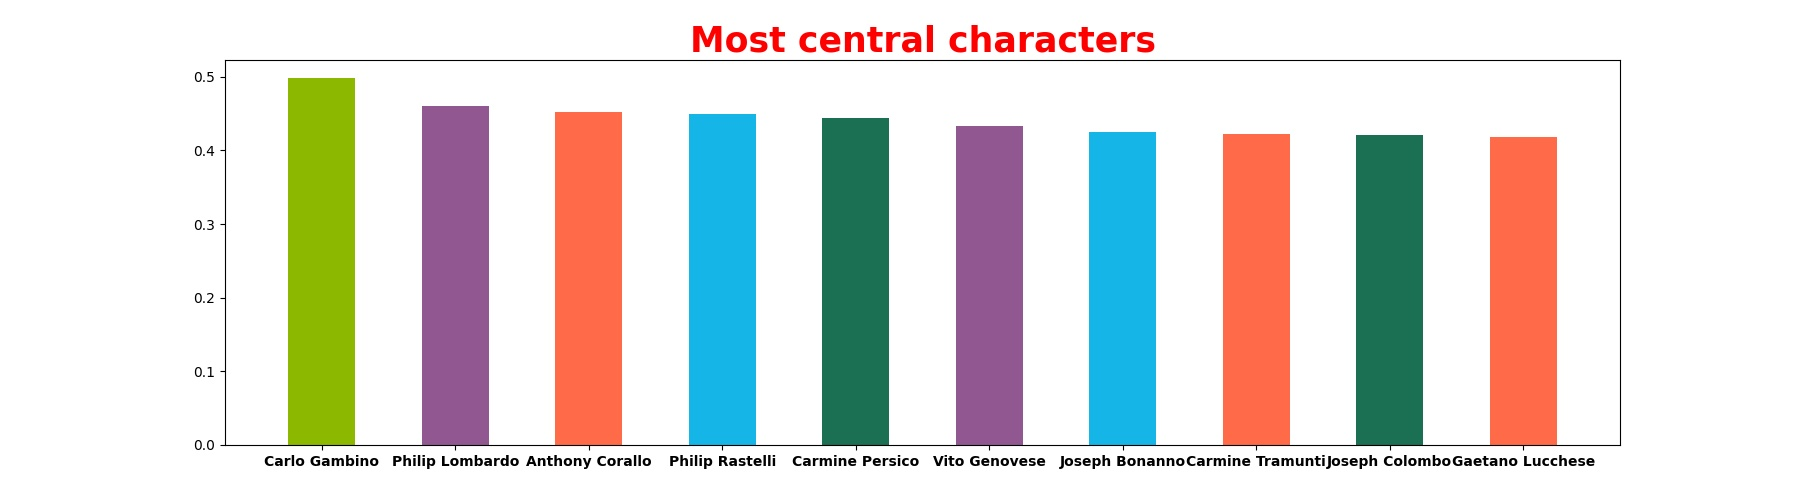
\includegraphics[width=675pt]{closeness.jpeg}
\end{figure}



%\vspace{20pt}
\noindent
As expected, this analysis returned different values and names from the previous one. In facts, we can see for the first time two members of the Colombo Family appearing, while Vincent Gigante, the most central character in the last analysis has gone. We can also see a smaller difference between each node, for instance:
\begin{itemize}
    \item \scalebox{1.3}{$\sigma_{degree}^2 $}$= 0.00115$ ; \scalebox{1.3}{$\sigma_{closeness}^2 $}$= 0.00053$
\end{itemize}
%\vspace{20pt}
By looking at these graphs, we can come to the conclusion that Philip Lombardo, Philip Rastelli and Carlo Gambino are the most central characters with more assurance, due to the fact that they appear on top of the chart with both a local and a collective measure of centrality. This result also shows that it is always best to cross different centrality measures in order to get a more valid result, as Vincent Gigante was the top contender for the main character position with the first analysis, but it "disappeared" in the second one.



\vspace{-20pt}
\textcolor{Titoli}{\subsection{Graph's structure}}
These results are based on a directed structure, where the information is supposed to come from the bottom of the hierarchy tree to the top, and from one boss to another. Keeping in mind this fact can help understand the values we got as centrality measures. It is obvious that, if the information could spread without an imposed direction, those values would be different, but the contenders would not change that much, because a family boss will always have more links and, most importantly, will always be the only person with an extra-family connection. One last way to structure our graph would be to link every family member with only one level of difference in the tree (for example a capo with an underboss but not a capo with a boss). This kind of network would allow a different spread of information, resulting in a completely different ranking for the most central characters.



\begin{figure}[t!]
\vspace{-250pt}
\centering
\includegraphics[width=600pt]{networkpic1.jpg}
\advance\leftskip-3.52cm
\end{figure}



\newpage
\pagecolor{white}\afterpage{\pagecolor{Pagine}}



\section{\textcolor{Paragrafi}{Degree Correlation}}
For the next step, we analyzed the degree correlation, in order to understand if our netwrork is assortative, disassortative or neutral. To do that, we calculated the value of $K_{nn}(k)$, which is the expected value of the degree of the neighbors of a node with degree $k$. We then built a loglogplot and found the value of $\mu$, which tells us how much inclined the line that approximates our chart is. 



\textcolor{Titoli}{\subsection{Program}}
In order to keep our program as interactive as possible, we also implemented a simple piece of code which can tell if the graph is assortative, disassortative or neutral just by the values of $\mu$. The main function is $k\_nearest\_neighbors()$. The code we used is the following:
\vspace{10pt}



\begin{figure}[h!]
\centering
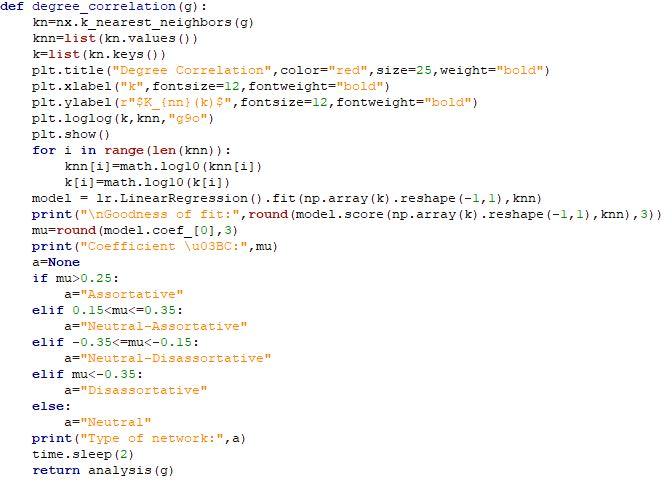
\includegraphics[width=400pt]{degreeprogram.JPG}
\advance\leftskip-1.52cm
\end{figure}



\textcolor{Titoli}{\subsection{Results}}
\noindent\begin{minipage}{0.5\textwidth}\raggedright
\textbf{Value of $\mu$: }-0.416\\
\textbf{Goodness of fit: }0.63\\
\textbf{Type of Network: }Disassortative
\end{minipage}%
\hfill%
\begin{minipage}{0.5\textwidth}
\vspace{-120pt}
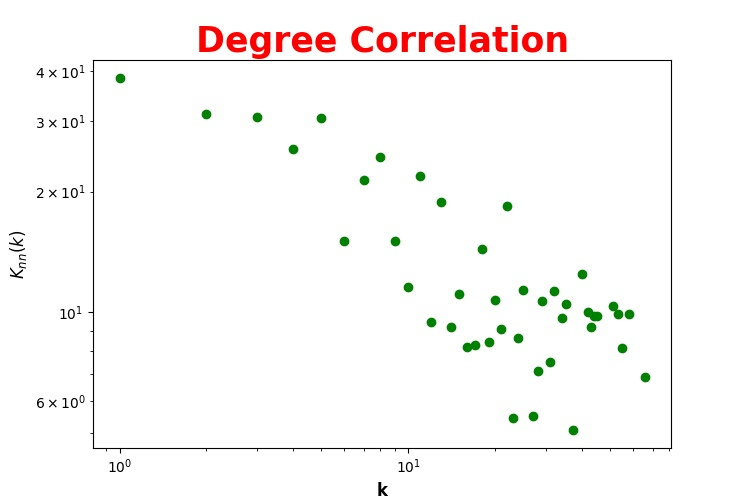
\includegraphics[width=300pt]{degreecorrelation.jpeg}
\end{minipage}
\newpage



\begin{figure}[t!]
\vspace{-250pt}
\centering
\includegraphics[width=600pt]{networkpic1.jpg}
\advance\leftskip-3.52cm
\end{figure}



\noindent
It is useful to remember that a network is assortative when his hubs tends to link each other, while when this does not happen, the network is disassortative. A network is neutral when it presents both these behaviours. Said that, our network is clearly disassortative. An easy way to know it is by looking at the value of $\mu$, which is smaller than 0 by some margin. We can also look at the graph in the previous page and see that it presents a negative inclination (given by the value of $\mu$). As we can imagine arrived at this point, this is another confirm that our network is Scale-Free and very robust, because by attacking one hub we do not immediately get to the next hub. If there was no connection between bosses of different families, the value of $\mu$ would have been very close to -1, but it is not the case. 



\section{\textcolor{Paragrafi}{Random failures and robustness}}
In order to analyze the network's robustness, we calculated the critical threshold beyond which the graph loses his connectedness. We let Python find the expected value of $k$ and $k^2$ and then the value of $\frac{\langle k^2\rangle}{\langle k\rangle}$, which is our threshold. The results are the following: \vspace{20pt}



\begin{table}[h!]
\centering
\begin{tabular}{|
>{\columncolor[HTML]{DAE8FC}}l |
>{\columncolor[HTML]{ECF4FF}}c |}
\hline
 & \multicolumn{1}{l|}{\cellcolor[HTML]{DAE8FC}\textbf{Critical Threshold}} \\ \hline
\textbf{Bonanno} & 0.930 \\ \hline
\textbf{Gambino} & 0.949 \\ \hline
\textbf{Colombo} & 0.929 \\ \hline
\textbf{Lucchese} & 0.940 \\ \hline
\textbf{Genovese} & 0.948 \\ \hline
\textbf{All the families} & 0.958 \\ \hline
\end{tabular}
\end{table}
\vspace{20pt}



\noindent
These values represent the percentage of nodes to cut off the graph in order to make him unconnected. The higher the graph's density, the higher his critical threshold. For instance, in order to make our graph unconnected, you have to remove nearly as much as 96\% of his nodes. Every value in the table is really high, a common property of the Scale-Free networks, which are known to be very robust to random failures, and so this is a further confirm that our network behaves as a Scale-Free. Let's analyze the family with the lowest value: the Colombo. If we climb back to the \hyperlink{Analysis}{Analysis}, we can see that the Colombo family has the least amount of nodes and links, while having two very central hubs in Carmine Persico and Joseph Colombo. Nevertheless, a value of 0.929 is nothing to worry about.\\
In the end, we can conclude by saying that each family is well defended against the loss of one of his members, which can be related both to his death and his imprisonment. It is surely not a coincidence: let's think of a real scenario for a random failure. The U.S. Government manages to capture a mobster from the Genovese Family. He is most likely to be a capo (if not a soldier, which is lower in the hierarchy tree) due to the pyramidal structure of the family (higher amount of lower-status individuals), and so he is in possess of less information compared to an underboss or a boss. This means that the boss (hub) is still safe, and the family with him.
\newpage



\pagecolor{white}



\begin{figure}[t!]
\vspace{-250pt}
\centering
\includegraphics[width=600pt]{networkpic1.jpg}
\advance\leftskip-3.52cm
\end{figure}



\section{\textcolor{Paragrafi}{Maximal Clique and Chromatic Number}}
In this short paragraph, we decided to include some information that are not strictly related to our analysis. First of all, it is useful to say that a clique is a subgraph in which each node is connected to every other node. The maximal clique is the clique with more nodes. This concept is strictly related to undirected graphs, but we managed to implement it in our graph due to the fact that we built a lot of multi directed edges, so that for example each boss is connected to each others both like a source and a target.



\begin{figure}[h!]
\centering
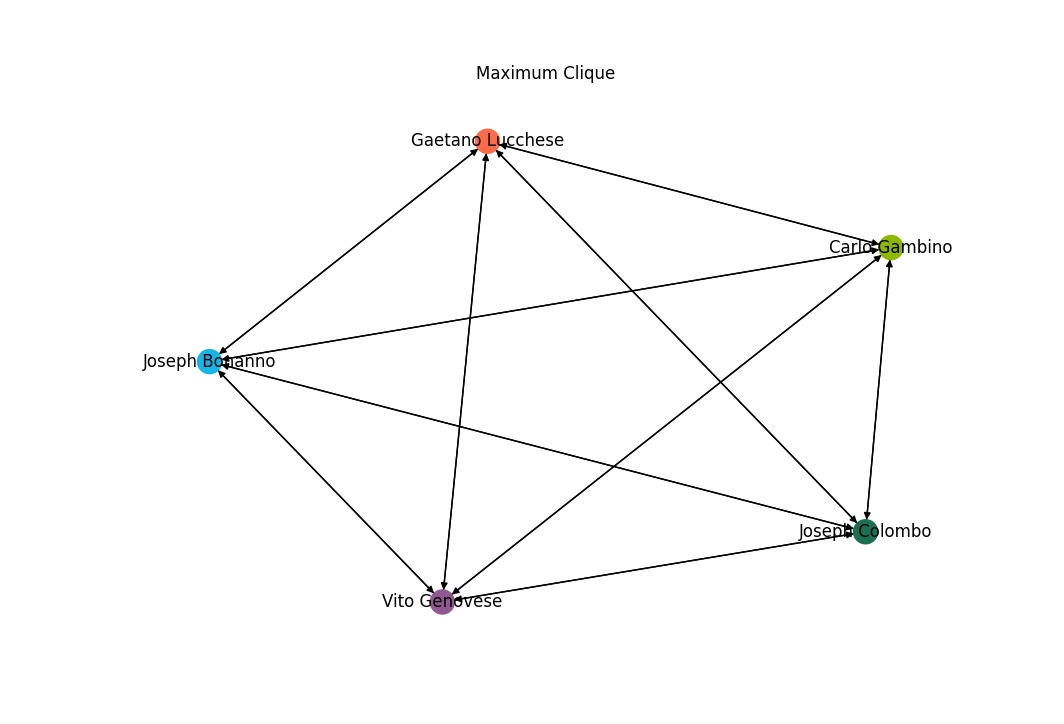
\includegraphics[width=500pt]{maximum_clique.jpeg}
\advance\leftskip-2.5cm
\end{figure}



\noindent
It is interesting to see that each node not only relates to a different family boss, but they are all related to the ones who gave their family its name. This clique was generated by Python, which draws each directed link as an arrow, and so each pair of nodes is connected by two arrows that behave like an undirected link. We then faced the coloring problem: how many colors do we need to color every node of the graph such as any adjacent node has different colors? It is clear that this problem is linked to the maximal clique, because for every clique each pair of nodes is adjacent to each other. For this reason, we could already know that there is a lower bound to the number of colors we need, which is 5, the dimension of the maximal clique. With a more precise analysis, we came to the conclusion that our graph's cromatic number is equal to 6. Keep in mind that these operations can be adapted to nearly every graph by using our \href{https://github.com/TizianoIannaccio/Network-Analytics}{Python code}. 



\begin{figure}[t!]
\vspace{-250pt}
\centering
\includegraphics[width=600pt]{networkpic1.jpg}
\advance\leftskip-3.52cm
\end{figure}



\section{\textcolor{Paragrafi}{Communities}}
The last aspect of the network to analize is the modularity. When a network presents distinct communities it has a value of modularity closer to 1. This means that in between each module there is a higher density, while between different modules there are fewer links. We already know that the only links between each family are the boss-boss edges. For this reason the expected result is to have around 5 modules that are structured as similar as possible to our families. For this operation we used Gephi, because we wanted an analysis from scratch, while NetworkX asks from which nodes the modularity algorithm should start. We obtained far more satisfactory results than expected:



\textcolor{Titoli}{\subsection{First Community (Bonanno)}}
\begin{figure}[h!]
\centering
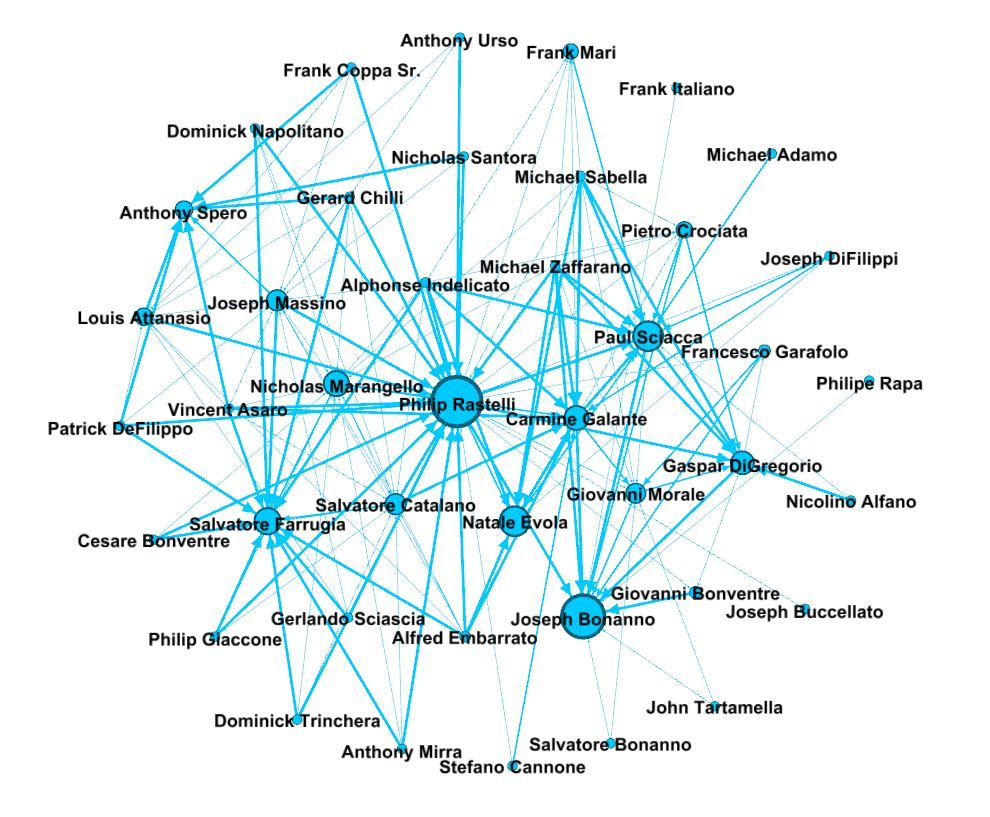
\includegraphics[width=450pt]{bonannomodule.JPG}
\advance\leftskip-1.5cm
\end{figure}



\noindent
These modules were filtered on Gephi based on the modularity coefficient. It is really hard to tell, as we will see with the \hyperlink{extramodule}{last module}, that there are a few nodes missing. This is great news, because it means that each family (as we will see) is nearly perfectly suitable to a single module. In facts, our graph's modularity coefficient is 0.763, a very high value.
\newpage



\begin{figure}[t!]
\vspace{-250pt}
\centering
\includegraphics[width=600pt]{networkpic1.jpg}
\advance\leftskip-3.52cm
\end{figure}



\textcolor{Titoli}{\subsection{Second Community (Gambino)}}
\begin{figure}[h!]
\vspace{35pt}
\centering
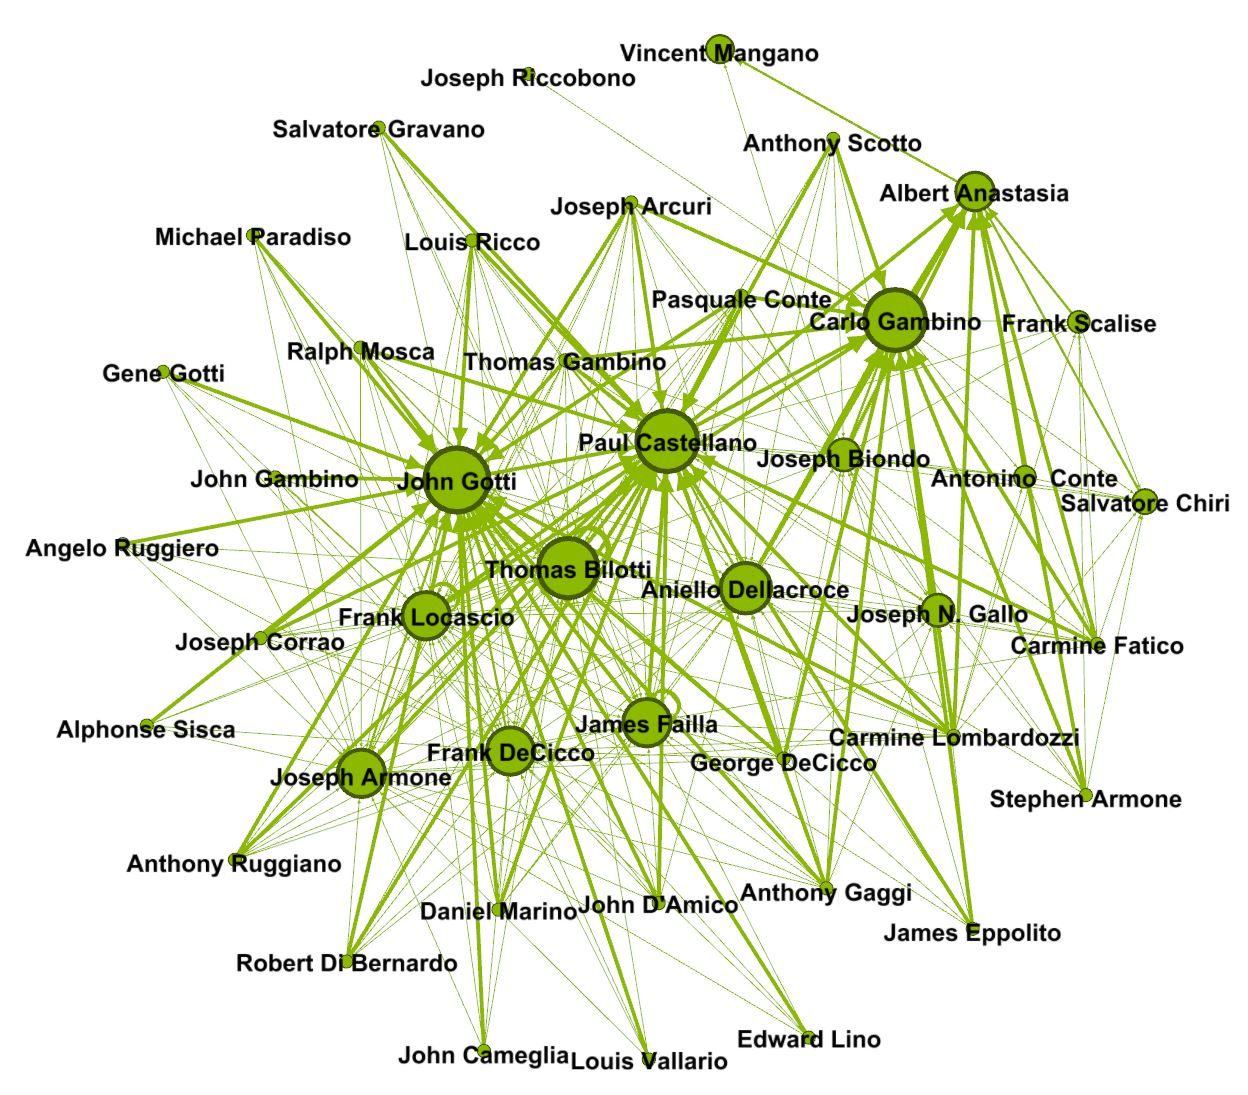
\includegraphics[width=550pt]{gambinomodule.JPG}
\advance\leftskip-2.5cm
\end{figure}
\newpage



\begin{figure}[t!]
\vspace{-250pt}
\centering
\includegraphics[width=600pt]{networkpic1.jpg}
\advance\leftskip-3.52cm
\end{figure}



\textcolor{Titoli}{\subsection{Third Community (Colombo)}}
\begin{figure}[h!]
\vspace{35pt}
\centering
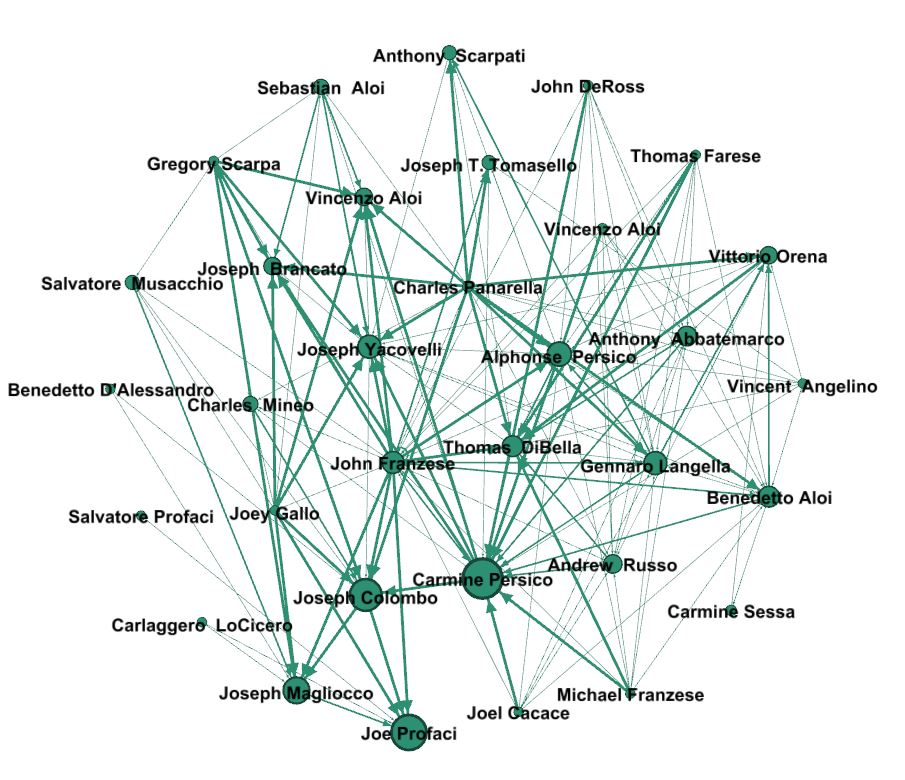
\includegraphics[width=550pt]{colombomodule.JPG}
\advance\leftskip-2.5cm
\end{figure}
\newpage



\begin{figure}[t!]
\vspace{-250pt}
\centering
\includegraphics[width=600pt]{networkpic1.jpg}
\advance\leftskip-3.52cm
\end{figure}



\textcolor{Titoli}{\subsection{Fourth Community (Lucchese)}}
\begin{figure}[h!]
\vspace{35pt}
\centering
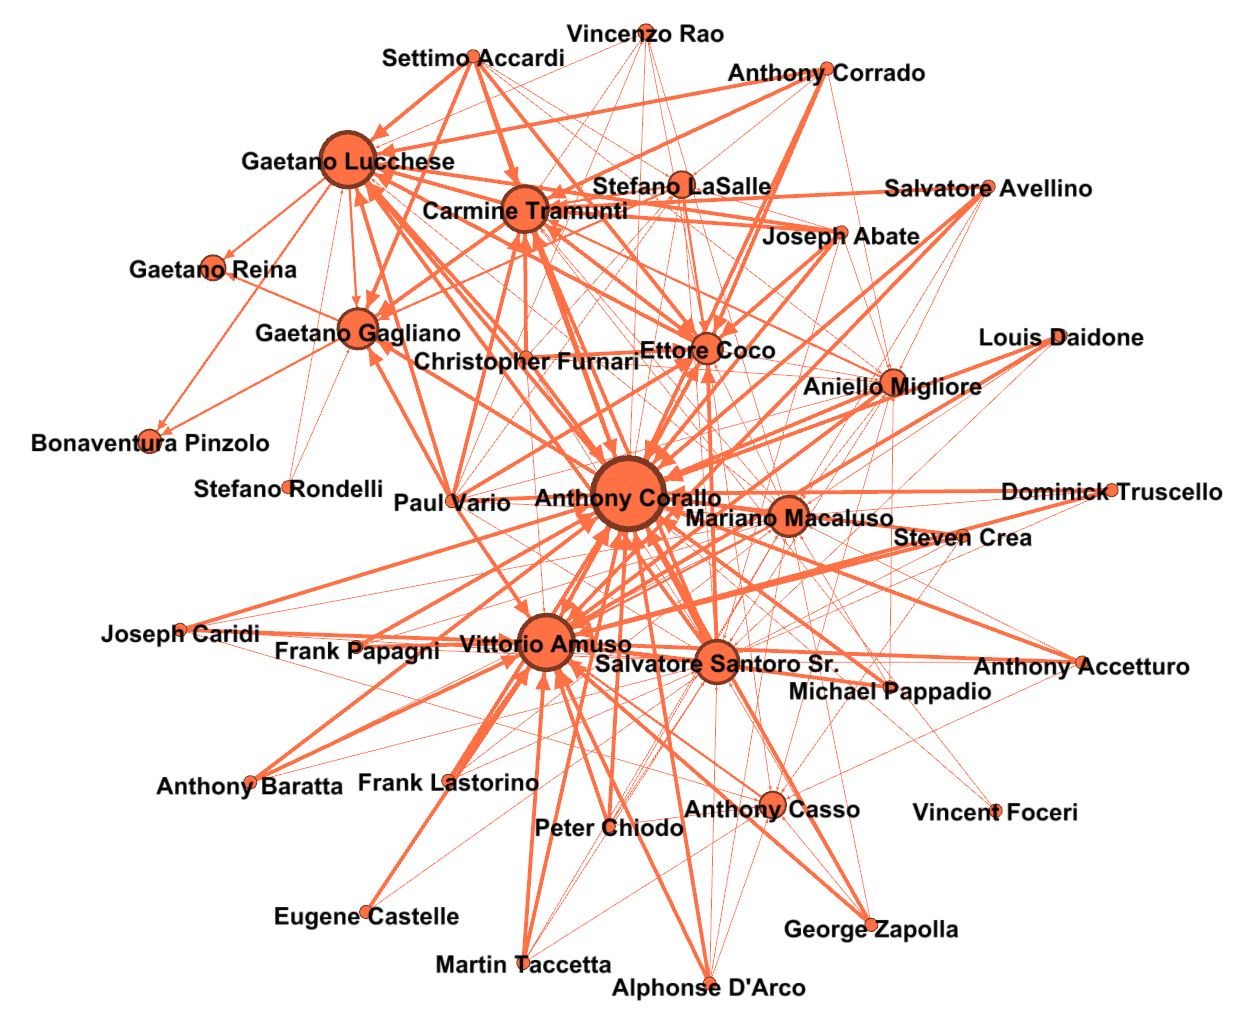
\includegraphics[width=550pt]{lucchesemodule.JPG}
\advance\leftskip-2.5cm
\end{figure}
\newpage



\begin{figure}[t!]
\vspace{-250pt}
\centering
\includegraphics[width=600pt]{networkpic1.jpg}
\advance\leftskip-3.52cm
\end{figure}



\textcolor{Titoli}{\subsection{Fifth Community (Genovese)}}
\begin{figure}[h!]
\vspace{35pt}
\centering
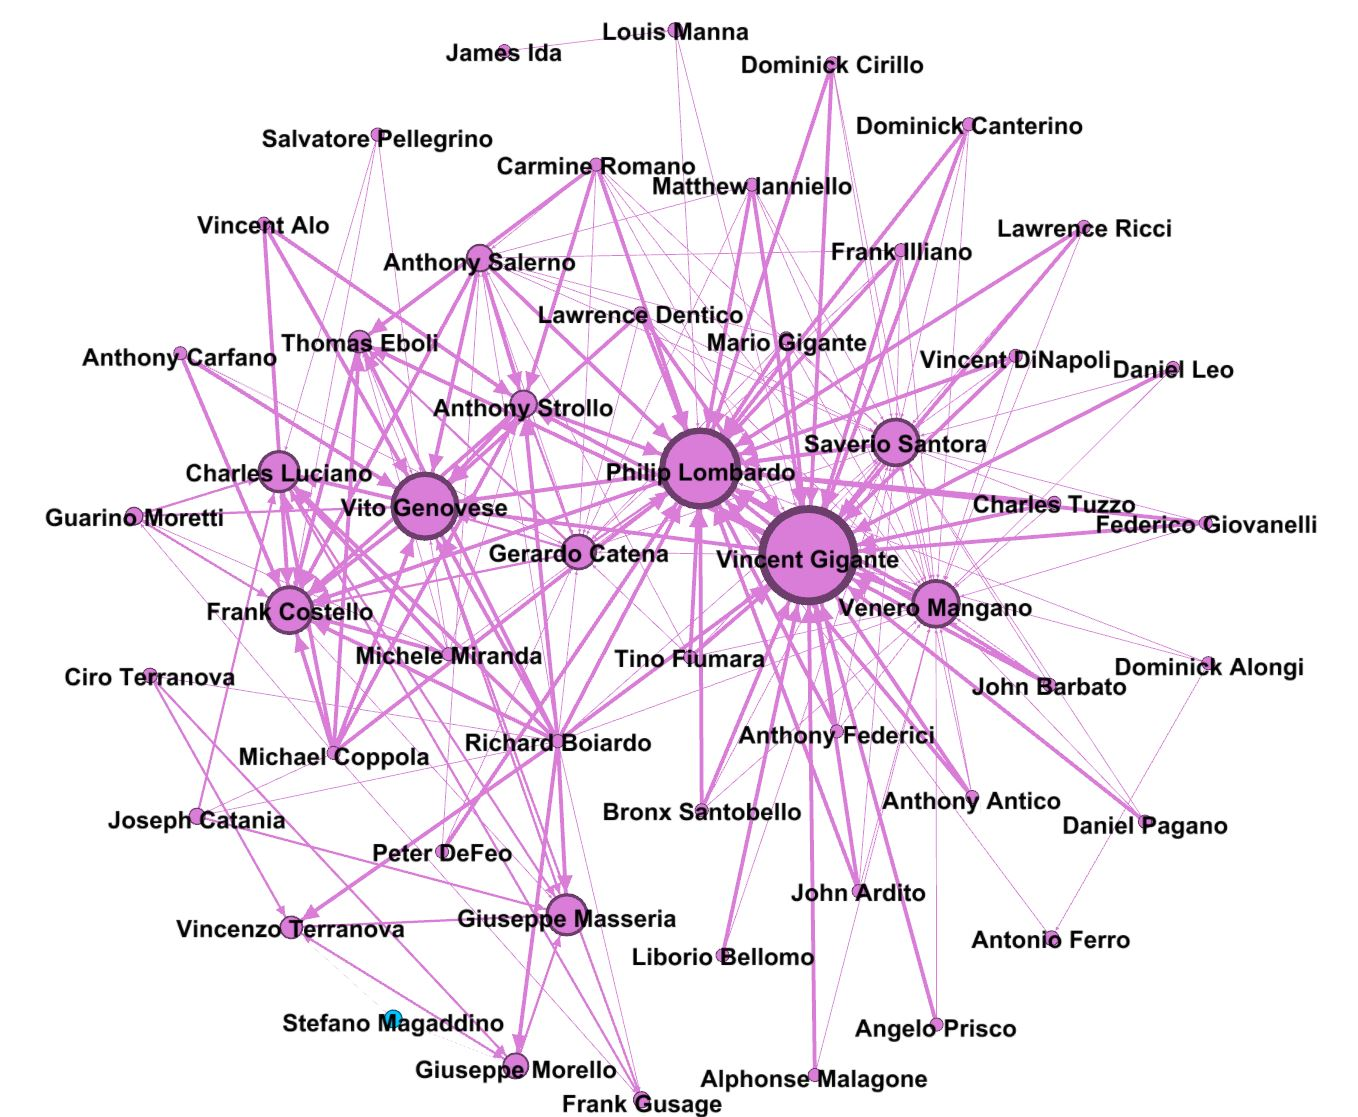
\includegraphics[width=550pt]{genovesemodule.JPG}
\advance\leftskip-2.5cm
\end{figure}
\newpage



\begin{figure}[t!]
\vspace{-250pt}
\centering
\includegraphics[width=600pt]{networkpic1.jpg}
\advance\leftskip-3.52cm
\hypertarget{extramodule}{}
\end{figure}


\textcolor{Titoli}{\subsection{Community Zero}}
\begin{figure}[h!]
\vspace{15pt}
\centering
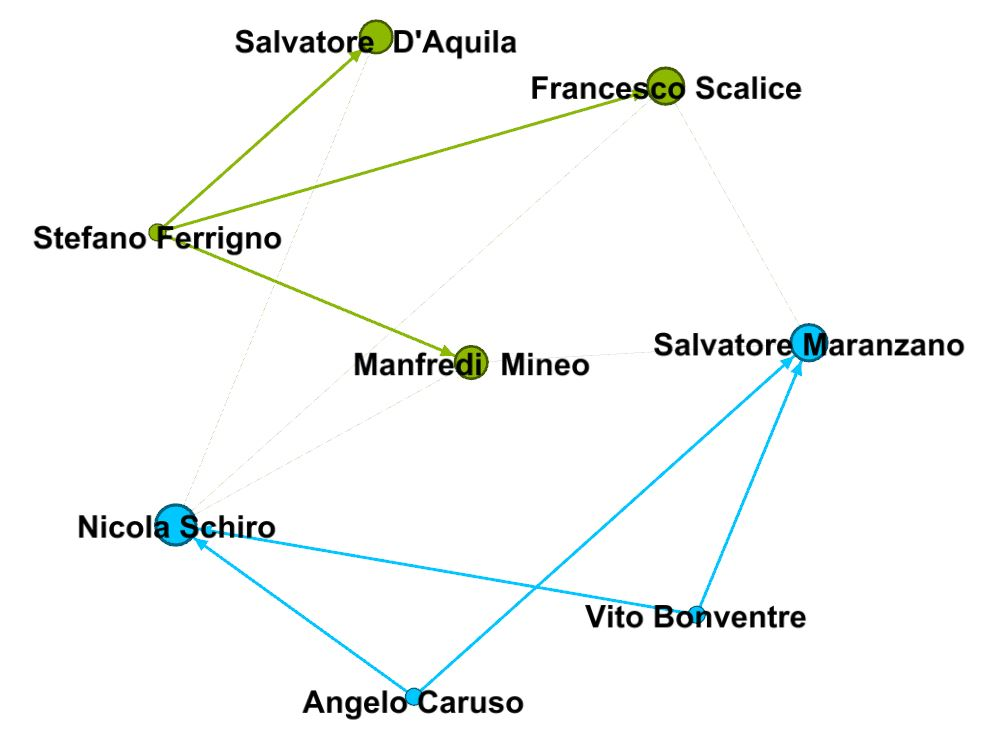
\includegraphics[width=500pt]{extramodule2.JPG}
\advance\leftskip-2cm
\end{figure}



\noindent
This extra community is composed by 4 members of the Gambino family and 4 members of the Bonanno family. There is another "outsider" node in the fifth community, which is Stefano Magaddino. This is due to tha fact that he has no links with his own family because we could not find any information about members of the Bonanno family when he was in charge of it (early 20's), and so he is only linked to bosses of other families in the same period of time. If we go back to the \hyperref[sec:Visualization]{Visualization}, we can see that each node of the Community Zero is not close to his own family, meaning that the layout-algorithm had already determined that their connections with their own family were weak.
\newpage



\begin{figure}[t!]
\vspace{-250pt}
\centering
\includegraphics[width=600pt]{networkpic1.jpg}
\advance\leftskip-3.52cm
\end{figure}



\pagecolor{Pagine}
\section{\textcolor{Paragrafi}{Conlclusions}}
Summing up, every aspect of our analysis tells us that our graph behaves as a Scale-Free network. It is now interesting to determine if, given the fact that we built ourselves the net, it can be interpreted as if it was pre-built and taken by an appropriate repository. It is not our job to determine that, but based on the results we obtained, we can at least say that the net does not present any abnormal behaviours, and can undergo any test we studied during our course. Furthermore, we can say that for every value we obtained during our analysis, we could find its cause in the structure of each family, or at least we could make an hypothesis on which real phenomenon could have generated such value. In conclusion, we can say that we are proud of the results we got.



\begin{figure}[h!]
\vspace{50pt}
\begin{flushright}

\includegraphics[width=125pt]{excel.png}
\end{flushright}
\end{figure}



\begin{figure}[h!]
\begin{flushright}

\includegraphics[width=125pt]{python.png}
\end{flushright}
\end{figure}



\begin{figure}[h!]
\begin{flushright}
\includegraphics[width=250pt]{Gephi.png}
\end{flushright}
\end{figure}



\end{document}
